% Author: Aditya Baradwaj, Rohan Suresh, Sukrit Arora
% Email: abaradwaj@berkeley.edu, rohansuresh@berkeley.edu, sukrit.arora@berkeley.edu

\qns{Change of Basis - Graphical}

\meta{Explain how a change of basis is simply another linear combination and how you are simply representing vectors with respect to a different reference.
}

\begin{enumerate}
\item A 'change of basis' refers to the process of taking a vector from one representation to another. Normally, we represent vectors in the standard unit basis. For example, we can write $\begin{bmatrix}3 \\ 5\end{bmatrix} = 3\begin{bmatrix}1 \\ 0\end{bmatrix} + 5\begin{bmatrix}0 \\ 1\end{bmatrix}$. But suppose we wanted to write $\begin{bmatrix}3 \\ 5\end{bmatrix}$ in a different way. Suppose we wanted to write it as a linear combination of $\begin{bmatrix}1 \\ 1\end{bmatrix}$ and $\begin{bmatrix}1 \\ -1\end{bmatrix}$. How would we do this? Can you express this as solving a system of linear equations? How about as solving a matrix-vector equation?

\ans{
That is equivalent to solving the system of equations $\begin{bmatrix}3 \\ 5\end{bmatrix} = \alpha\begin{bmatrix}1 \\ 1\end{bmatrix} + \beta\begin{bmatrix}1 \\ -1\end{bmatrix}$. Therefore, we want $\alpha + \beta = 3$ and $\alpha - \beta = 5$. Solving, we get that $\alpha = 4$ and $\beta = -1$.

Written as a matrix-vector equation, this is:
$$
\begin{bmatrix}
1 & 1 \\
1 & -1 \\
\end{bmatrix}
\begin{bmatrix}\alpha \\ \beta \end{bmatrix} = \begin{bmatrix}3 \\ 5 \end{bmatrix}
$$
}

\item Suppose that you have some vector $\vec{x} \in \R^n$ and you want to put it in the basis defined by the set of vectors $\{\vec{v_1}, \ldots, \vec{v}_n\}$. Give a general equation that would allow you to do this.

\ans{
Let us define the matrix $\m{V} = \begin{bmatrix}
\vec{v_1} & \vec{v_2}
\end{bmatrix}$.
We want to solve the system of equations
$$Vy = x$$
Here, $y$ is the variable we are solving for. Note that $V$ must be invertible, since the set of vectors form a basis (and therefore, they are linearly independent). Multiplying by $V^{-1}$, we get:
$$y = V^{-1}x$$
}

\item { Let us use the subscript $V$ to refer to a vector or matrix in the basis $\m{V}$. We want to find the matrix $\m{A_V}$ such that $\m{A_V}\vec{x_V} = (\m{A}\vec{x})_V$. That is, we want the matrix $\m{A_V}$ to act the same way in the $V$ basis that the matrix $A$ would act in the standard basis.
}

\ans{
For all $\vec{x}$,
\begin{flalign*}
& \m{A_V}\vec{x_V} = (\m{A}\vec{x})_V &\\
& \implies \m{A_V} (V^{-1}\vec{x}) = (V^{-1}\m{A}\vec{x}) &\\
& \implies V \m{A_V} V^{-1}\vec{x} = \m{A}\vec{x} &\\
& \implies (V \m{A_V} V^{-1}) \vec{x} = \m{A}\vec{x} &\\
& \implies V \m{A_V} V^{-1} = \m{A} \text{ (If 2 matrices give the same output for all input vectors, they must be the same)} &\\
& \implies \m{A_V} = V^{-1} \m{A} V &\\
\end{flalign*}
}

\item Now that we know how to take a vector or matrix in the standard basis and represent it in a different basis, how can we take a vector $\vec{x}$ in the basis $\{\vec{a_1}, \ldots, \vec{a_n}\}$ and find its representation in the basis ${\vec{b_1}, \ldots, \vec{b_n}}$?

\ans{
First, we go from basis $\m{A}$ to the standard basis, and then from the standard basis to basis $\m{B}$.
}

\item Now let's consider the vector $\begin{bmatrix}1 \\ 1\end{bmatrix}$ in the standard basis. Find its representation in the basis of a rotation matrix for $\theta = 45^{\circ}$. Graph the original vector and the vector in the new basis. For reference, the rotation matrix of an angle $\theta$ is
$
\begin{bmatrix}
cos\theta & -sin\theta \\
sin\theta & cos\theta \\
\end{bmatrix}
$.

\begin{center}
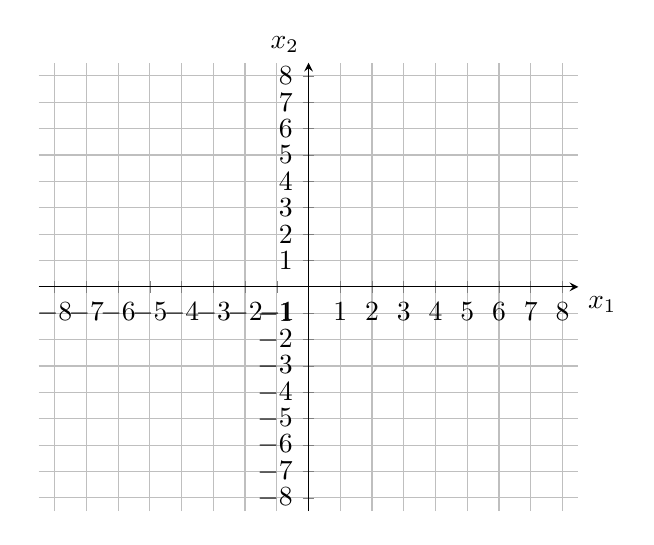
\begin{tikzpicture}[>=latex]
\begin{axis}[
  axis x line=center,
  axis y line=center,
   xtick={-8,...,8},
  ytick={-8,...,8},
  xlabel={$x_1$},
  ylabel={$x_2$},
  xlabel style={below right},
  ylabel style={above left},
  xmin=-8.5,
  xmax=8.5,
  ymin=-8.5,
  ymax=8.5,
  grid]
\end{axis}
\end{tikzpicture}
\end{center}

\ans{
First, let's evaluate the rotation matrix at $\theta = \frac{\pi}{4} $ 
$$
\mathbf{R} =
\begin{bmatrix}
cos\theta & -sin\theta \\
sin\theta & cos\theta \\
\end{bmatrix}
 = \begin{bmatrix}
\frac{\sqrt{2}}{2} & -\frac{\sqrt{2}}{2} \\
\frac{\sqrt{2}}{2} & \frac{\sqrt{2}}{2} \\
\end{bmatrix}$$

Then, we can set up the equation described in part (b)

$$
\mathbf{R}\vec{y}=\begin{bmatrix} 1 \\ 1 \end{bmatrix}
$$

$$
\vec{y} = R^{-1}\begin{bmatrix} 1 \\ 1 \end{bmatrix}
$$
We can see that the inverse of a rotation matrix is that same matrix evaluated at $\theta = -\frac{\pi}{4}$. So, $\mathbf{R}^{-1} = \begin{bmatrix}
\frac{\sqrt{2}}{2} & \frac{\sqrt{2}}{2} \\
-\frac{\sqrt{2}}{2} & \frac{\sqrt{2}}{2} \\
\end{bmatrix}$

So, we can see that $$\vec{y}=\begin{bmatrix}
\frac{\sqrt{2}}{2} & \frac{\sqrt{2}}{2} \\
-\frac{\sqrt{2}}{2} & \frac{\sqrt{2}}{2} \\
\end{bmatrix}\begin{bmatrix} 1 \\ 1 \end{bmatrix}=\begin{bmatrix} \sqrt{2} \\ 0 \end{bmatrix}$$
}

\item Suppose that your set of vectors ${v_1, \ldots, v_n}$ is linearly dependent (meaning that it cannot be a basis). Is it still possible to take any vector $\vec{x}$ and write it as a linear combination of these vectors? Justify your answer from a matrix-vector equation point of view, and from a graphical point of view.


\ans{
No, it is not possible. From a matrix equation point of view, we know that the matrix $V$ from the previous part cannot be invertible, since it has linearly dependent columns. From a graphical point of view, we know that these vectors span some subspace of $\mathbf{R}^n$ which is smaller in dimension. So, it will not be possible for us to represent any vector outside that subspace as a linear combination of vectors in the set.
}

\end{enumerate}